\subsection{Initial parameters and approach \label{sec:param_approach}}
Once the algorithm is written, some initial parameters must be choosen. Here : the number of iterations, that we will note $n$, and the parameter of trade-off between explotation and exploration, that we will note $p$. As the performance of the AI will depend on those, an initial choice was made, arbitrarily, and depending on the behaviour and performance of the AI, they have been modified. \\

The most important conclusion that was pointed out was the fact that the iterations must be \textbf{as fast as possible}, because the more $n$ can grow, the better. This means that the initial \textbf{implementation of the game} must be rethought if it is not optimized for being as fast as possible. Then, during the execution of the algorithm, some \textbf{slow methods} must be avoided, e.g. \code{deepcopy}. Avoid some redundant calls to functions, etc. \\

With such cleaning of the algorithm, the AI went from 20 seconds by move with $n=200$ to 20 seconds by move with $n=20k$. Note that the documentation about MCTS informs us that having relatively small $n$, like $n=200$, will result in an AI playing randomly. \\

$n$ is a parameter that tells how much the tree is "studied" : we want a tree with the highest $n$ possible for a realistic time. On the other hand, $p$ tells us about the way the tree is going to be used. 
\begin{itemize}
    \item Small $p$ : exploration has a privilege 
    \item Big $p$ : explotation has a privilege 
\end{itemize}

Hence, once $n$ was set to being the biggest possible for realistic execution time, $p$ can be tweaked to have a smarter AI : should we explore more, or exploit more ? This will depend on the AI's performance for each $p$, and will be discussed in the next sections.

\subsection{Benchmark setup and implementation}
To analyze the performance of the AI, the following tests were conducted. $4$ values of $n$ were tested, and $8$ values of $p$. They can be seen on table \ref{table:benchmark_values}. For each combination, 10 games were simulated, giving a total of $8\times4\times10 = 320$ simulations, that took about 26 hours to run.
\begin{table}[h]
    \centering
    \begin{tabular}{|c|}
        \hline 
        $n$ \\
        \hline
        5000 \\
        10000 \\
        15000 \\
        20000 \\
        \hline
    \end{tabular}
    \begin{tabular}{|c|}
        \hline 
        $p$ \\
        \hline
        0.25 \\
        0.5 \\
        0.75 \\
        1 \\
        1.25 \\
        1.5 \\
        1.75 \\
        2 \\
        \hline
    \end{tabular}
    \caption{Test values for $n$ and $p$.}
    \label{table:benchmark_values}
\end{table}

The implementation can be found in the \code{benchmark.py} file.
\subsection{Wins and losses}
From the 320 simulations, we found nothing to conclude on the performance on the AI on its winning ability. There are 6 wins out of those 320 games, and the rest are draws and losses\footnote{The initial implementation of Minimax thinks that it is winning as long as it has more pieces left, and the game ends up by drawing.} \\

From this, we conclude that no matter the value of $p$, the MCTS AI can still not find its path to victory, and that $n$ should therefore be improved, by optimizing the run in the initial implementaion, or finding another way to speed up the process (as will be discussed later).

\subsection{Execution time behaviour depending on the parameters}
In this section, we answer to the following questions to understand the reaction of the execution time in result to modifying the parameters :
\begin{itemize}[label=$\blacktriangleright$]
    \item How does $t$ react when increasing $n$ ? Linearly ? Exponentially ? This is answered on figure \ref{fig:benchmark-n_bplot}.
    \item Does $p$ have an influence on the execution time ? Answered on figure \ref{fig:benchmark-p_bplot}.
\end{itemize}
\begin{figure}[h]
    \centering
    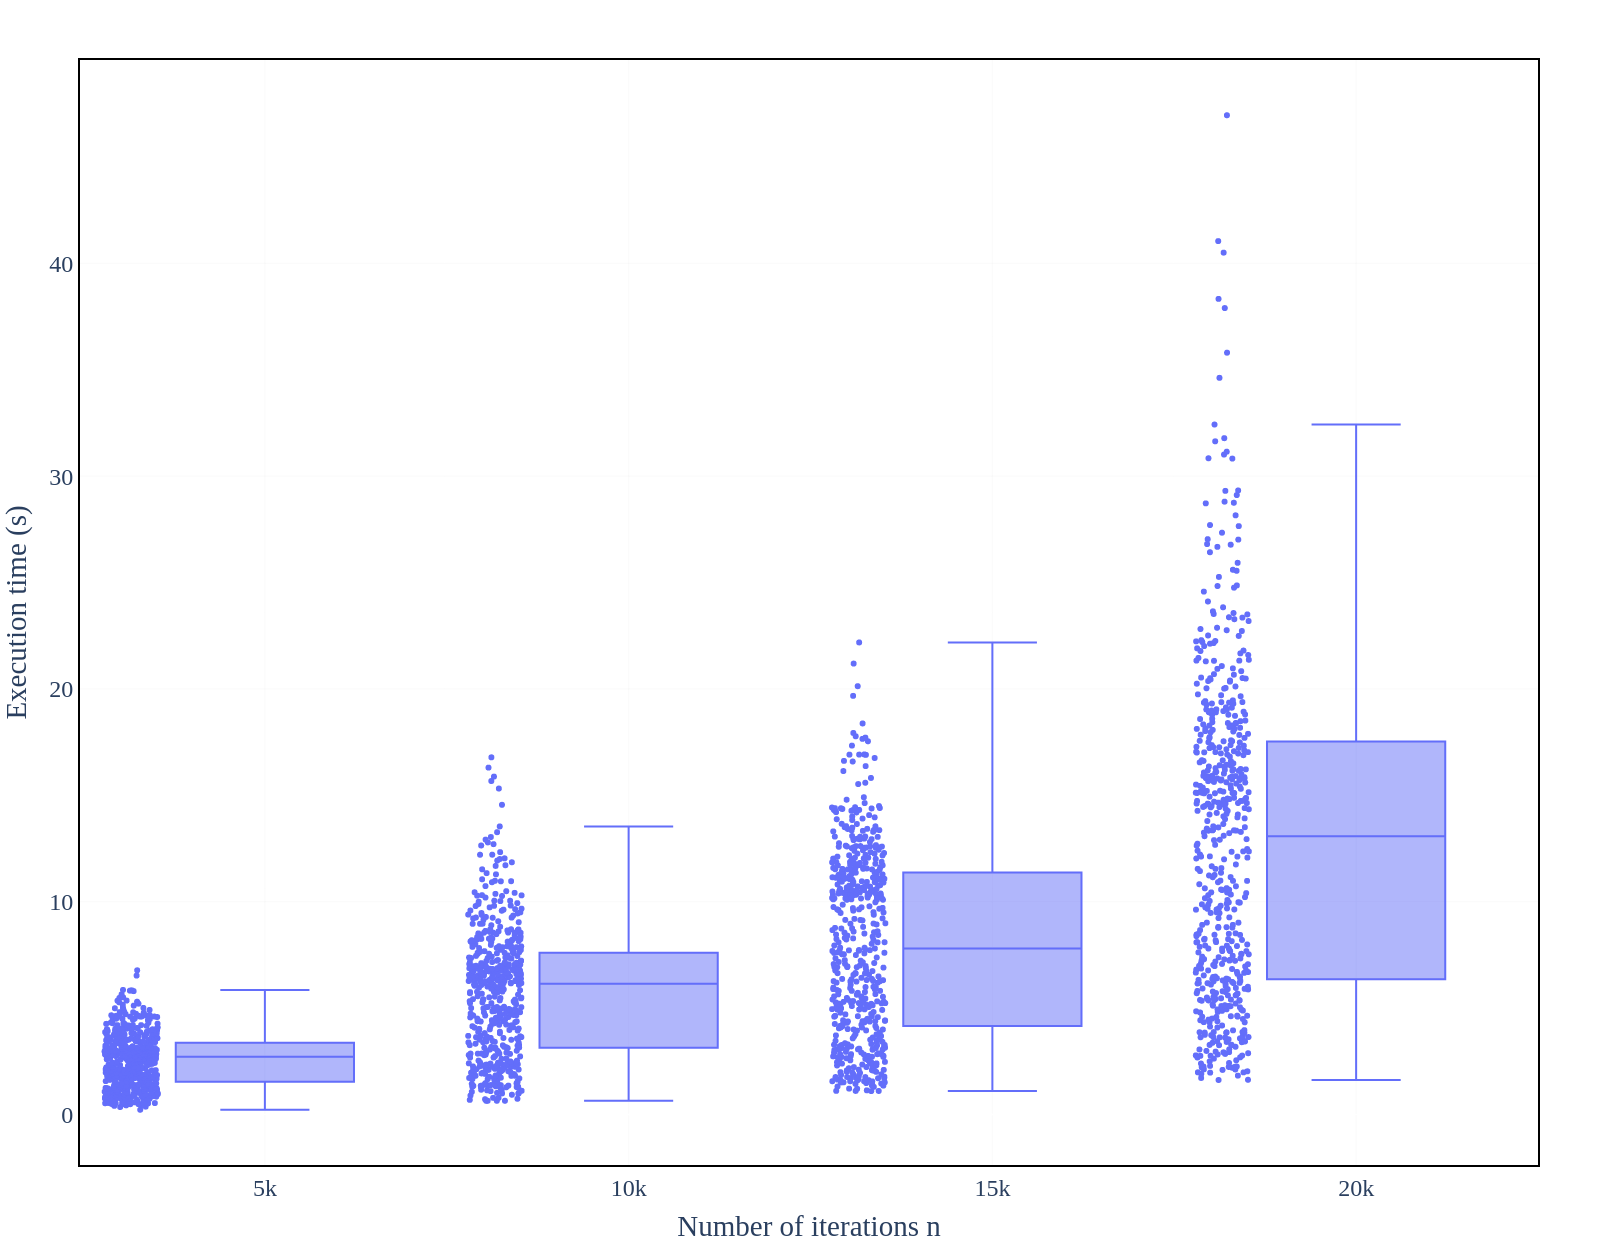
\includegraphics[width=\linewidth]{n_box_plot.png}
    \caption{Box-plot of the execution time (in seconds) with several values of $n$, for $p=4$. A linear dependance can be seen for the median.}
    \label{fig:benchmark-n_bplot}
\end{figure}
\begin{figure}[h]
    \centering
    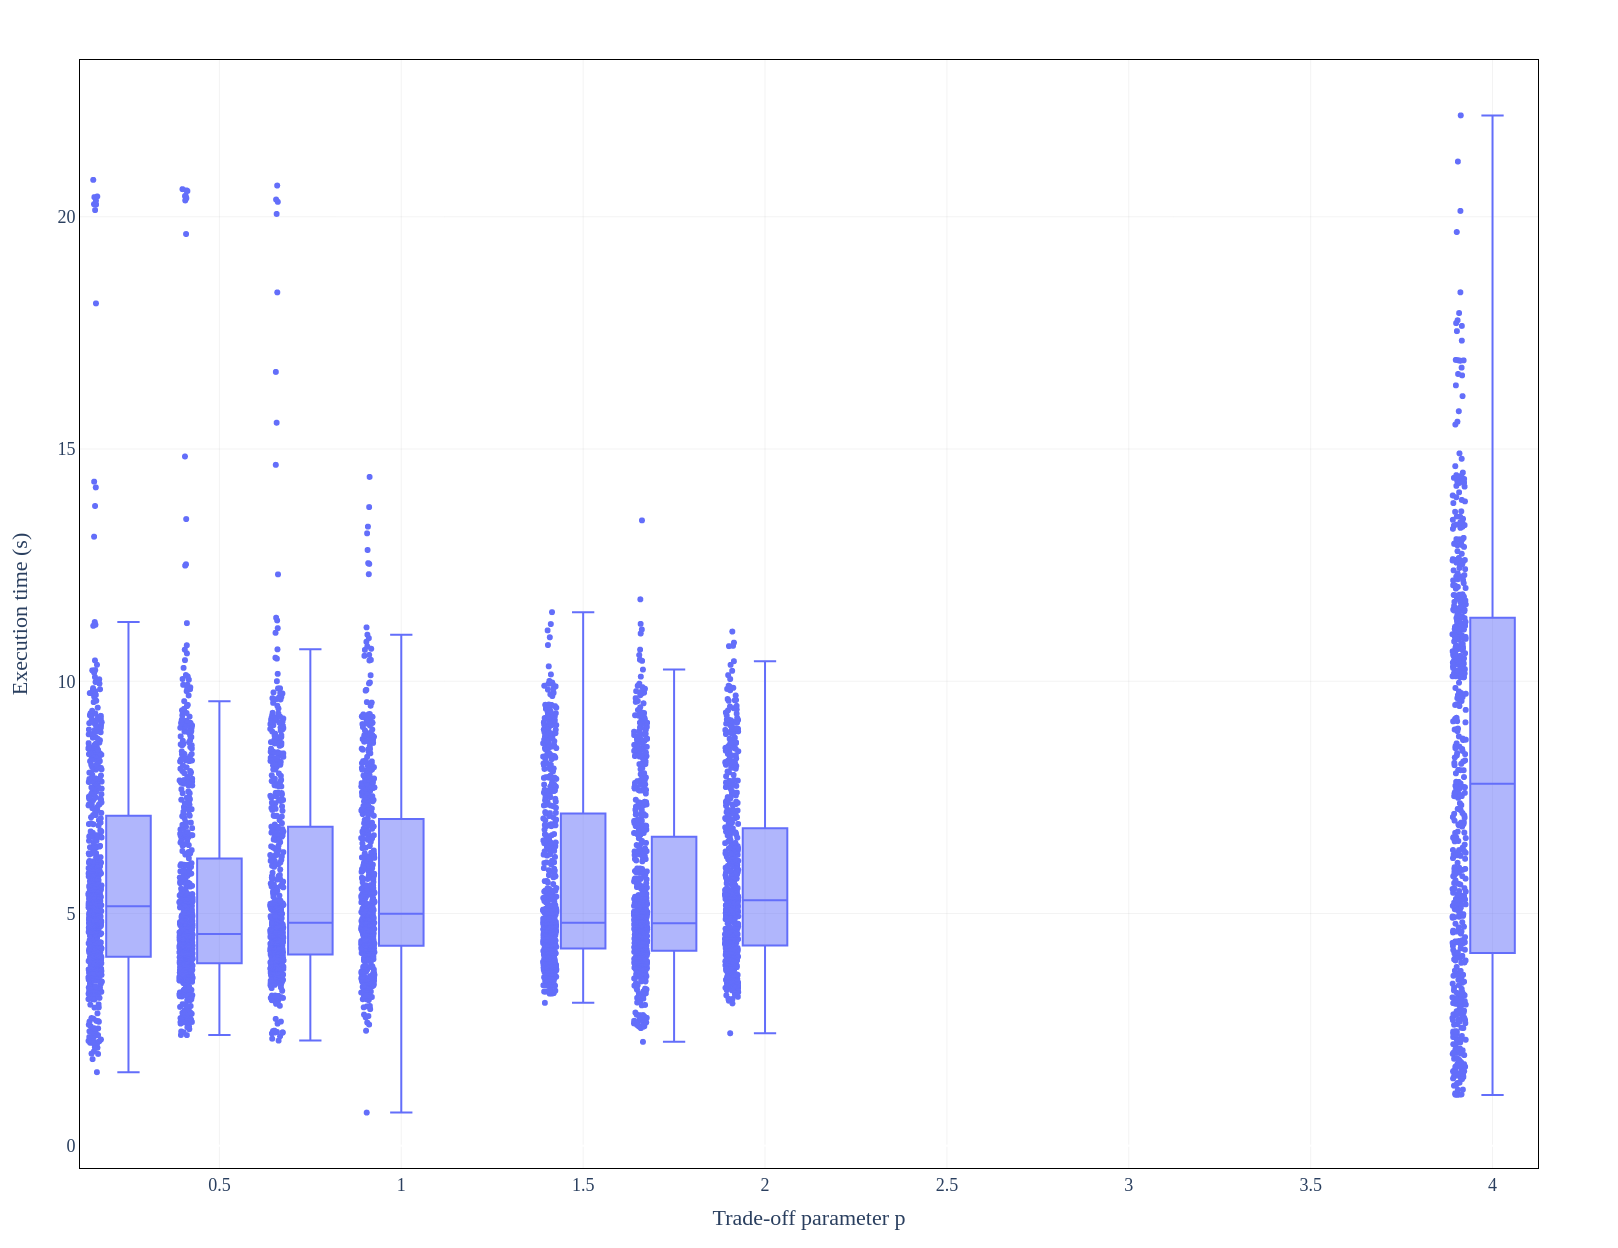
\includegraphics[width=\linewidth]{p_box_plot.png}
    \caption{Box-plot of the execution time (in seconds) with several values of $p$, for $n=15k$. As expected, the average execution time does not depend on $p$, hence is constant, although it seems like the execution time seems to spread for high $p$.}
    \label{fig:benchmark-p_bplot}
\end{figure}